% This must be in the first 5 lines to tell arXiv to use pdfLaTeX, which is strongly recommended.
\pdfoutput=1
% In particular, the hyperref package requires pdfLaTeX in order to break URLs across lines.

\documentclass[11pt]{article}

% Change "review" to "final" to generate the final (sometimes called camera-ready) version.
% Change to "preprint" to generate a non-anonymous version with page numbers.
% \usepackage[review]{acl}
\usepackage[final]{acl}

% Standard package includes
\usepackage{times}
\usepackage{latexsym}

% For proper rendering and hyphenation of words containing Latin characters (including in bib files)
\usepackage[T1]{fontenc}
% For Vietnamese characters
% \usepackage[T5]{fontenc}
% See https://www.latex-project.org/help/documentation/encguide.pdf for other character sets

% This assumes your files are encoded as UTF8
\usepackage[utf8]{inputenc}

% This is not strictly necessary, and may be commented out,
% but it will improve the layout of the manuscript,
% and will typically save some space.
\usepackage{microtype}

% This is also not strictly necessary, and may be commented out.
% However, it will improve the aesthetics of text in
% the typewriter font.
\usepackage{inconsolata}

%Including images in your LaTeX document requires adding
%additional package(s)
\usepackage{graphicx}

% If the title and author information does not fit in the area allocated, uncomment the following
%
%\setlength\titlebox{<dim>}
%
% and set <dim> to something 5cm or larger.

\title{NLP 2025 Lab 1 Report: Tokenization}

% Author information can be set in various styles:
% For several authors from the same institution:
% \author{Author 1 \and ... \and Author n \\
%         Address line \\ ... \\ Address line}
% if the names do not fit well on one line use
%         Author 1 \\ {\bf Author 2} \\ ... \\ {\bf Author n} \\
% For authors from different institutions:
% \author{Author 1 \\ Address line \\  ... \\ Address line
%         \And  ... \And
%         Author n \\ Address line \\ ... \\ Address line}
% To start a separate ``row'' of authors use \AND, as in
% \author{Author 1 \\ Address line \\  ... \\ Address line
%         \AND
%         Author 2 \\ Address line \\ ... \\ Address line \And
%         Author 3 \\ Address line \\ ... \\ Address line}

\author{First Author \\
  Affiliation / Address line 1 \\
  \texttt{email@domain} \\\And
  Second Author \\
  Affiliation / Address line 1 \\
  \texttt{email@domain} \\\And
  Third Author \\
  Affiliation / Address line 1 \\
  \texttt{email@domain} \\}

%\author{
%  \textbf{First Author\textsuperscript{1}},
%  \textbf{Second Author\textsuperscript{1,2}},
%  \textbf{Third T. Author\textsuperscript{1}},
%  \textbf{Fourth Author\textsuperscript{1}},
%\\
%  \textbf{Fifth Author\textsuperscript{1,2}},
%  \textbf{Sixth Author\textsuperscript{1}},
%  \textbf{Seventh Author\textsuperscript{1}},
%  \textbf{Eighth Author \textsuperscript{1,2,3,4}},
%\\
%  \textbf{Ninth Author\textsuperscript{1}},
%  \textbf{Tenth Author\textsuperscript{1}},
%  \textbf{Eleventh E. Author\textsuperscript{1,2,3,4,5}},
%  \textbf{Twelfth Author\textsuperscript{1}},
%\\
%  \textbf{Thirteenth Author\textsuperscript{3}},
%  \textbf{Fourteenth F. Author\textsuperscript{2,4}},
%  \textbf{Fifteenth Author\textsuperscript{1}},
%  \textbf{Sixteenth Author\textsuperscript{1}},
%\\
%  \textbf{Seventeenth S. Author\textsuperscript{4,5}},
%  \textbf{Eighteenth Author\textsuperscript{3,4}},
%  \textbf{Nineteenth N. Author\textsuperscript{2,5}},
%  \textbf{Twentieth Author\textsuperscript{1}}
%\\
%\\
%  \textsuperscript{1}Affiliation 1,
%  \textsuperscript{2}Affiliation 2,
%  \textsuperscript{3}Affiliation 3,
%  \textsuperscript{4}Affiliation 4,
%  \textsuperscript{5}Affiliation 5
%\\
%  \small{
%    \textbf{Correspondence:} \href{mailto:email@domain}{email@domain}
%  }
%}

\begin{document}
\maketitle
\begin{abstract}
DELETE (OR REPLACE) AFTER YOU READ. This is a template for the report of the NLP 2025 labs. It is adapted from the Association for Computational Linguistics (ACL) conference\footnote{\url{https://aclrollingreview.org/authors}}. Fill in your names in the authors list and provide your answers to the exercises listed in the accompanying notebook. The answer to each exercise should be in a separate section. For the coding exercises, provide code snipped and a short explanation. For the open questions, you can add figures, plots, tables, etc. Make sure to include a short discussion.

You need to submit a PDF of your report (use the templates provided in latex (preferred) or word and a copy of your notebook with the code. Make sure that all figures/results/plots are shown in your (execucted) notebook. While you may talk with others about this lab, we ask that you write your solutions with your group only. If you do discuss specific tasks with others please include their names in the appendix. Honor code applies to this lab. For more check Syllabus §7.2. It is mandatory to list and disclose any website (or other resource) you used (e.g. stackoverflow) as well as any genAI tools (e.g. chatGPT) used. Failure to disclose these is a violation of academic integrity. For more check Syllabus §7.3. THIS TEXT WILL BE SELF-DESTROYED AFTER YOU READ IT.
\end{abstract}

\section*{Uesful \LaTeX{} commands}
In this short section we will show you several commands that you can adapt when writing your answers. Feel free to remove this section before submitting your report.

To write a short in-line code snippet you can use the following command \verb|print('Hello World')|. For longer pieces of code use the following:
\begin{quote}
\begin{verbatim}
def foo():
    print('Hello World')
\end{verbatim}
\end{quote}

Here is the example of a table. Each table and figure should have a reference from text. You can set the label in the table and use \verb|\ref{tab:citations}| command to reference it. For example, Table~\ref{tab:citations} presents different ways to cite a bibliography. In the report, you can add references but it is not required.

\begin{table}
  \centering
  \begin{tabular}{lll}
    \hline
    \textbf{Output}           & \textbf{natbib command} \\
    \hline
    \citep{Gusfield:97}       & \verb|\citep|           \\
    \citet{Gusfield:97}       & \verb|\citet|           \\
    \hline
  \end{tabular}
  \caption{\label{citation-guide}
    Citation commands supported by the style file.
    The style is based on the natbib package and supports all natbib citation commands.
  }
  \label{tab:citations}
\end{table}

Figures can be added by first uploading the image file to overleaf and then using the following command (and reference it using Figure~\ref{fig:zipf}):
\begin{figure}[t]
  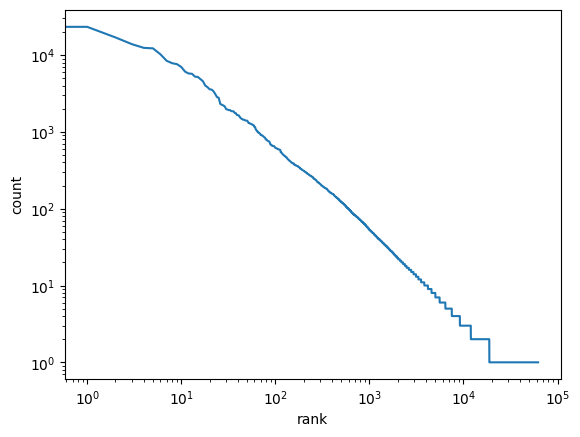
\includegraphics[width=\columnwidth]{zipf.png}
  \caption{This is a caption of the figure.}
  \label{fig:zipf}
\end{figure}

\section{Exercise 1: Questions about the datasets}

Your answers here.

% \subsection{What is the size of the training, test and validation datasets?}

% Your answer here

% \subsection{What are the top 5 most frequent emojis in the validation dataset?}

% \subsection{Compare the distributions of labels (emojis) between training and validation datasets.}

% \subsection{How many examples with the "fire" emoji are in the training dataset?}

% \subsection{What is the average length (in characters) of the tweets in the training dataset?}

\section{Exercise 2: Write the text cleaning function}

\section{Exercise 3: Build the vocabulary}

\section{Exercise 4: Frequency of pairs of words}

\section{Exercise 5: Tokenize the dataset}

\section{Exercise 6: Questions about the tokenization}

\section{Exercise 7: Counting the characters}

\section{Exercise 8: Calculate the frequency statistics of adjacent symbol pairs}

\section{Exercise 9: BPE algorithm}

\section{Exercise 10: Comparing tokenizers}

% Bibliography entries for the entire Anthology, followed by custom entries
%\bibliography{anthology,custom}
% Custom bibliography entries only

\bibliography{custom}

\appendix

\section{Collaborators outside our group}



\section{Use of genAI}

Use of genAI tools (e.g. chatGPT), websites (e.g. stackoverflow): list websites where you found code (or other info) as well as include information on how you used genAI tools (e.g. prompts).  Failure to disclose use of genAI tools is violation of adademic integrity.

% This is an appendix.

\end{document}
